\documentclass[a5paper]{article}

% Uncomment the following line to allow the usage of graphics (.png, .jpg)
%\usepackage[pdftex]{graphicx}
% Comment the following line to NOT allow the usage of umlauts

\pagestyle{empty}
\usepackage[T2A]{fontenc}
\usepackage[utf8]{inputenc}
\usepackage[russian]{babel}
\usepackage{cmap}
\usepackage{amsthm}
\usepackage{amsmath}
\usepackage{units}
\usepackage{fancyhdr}
\usepackage{forloop}
\usepackage{amssymb}
\usepackage{url}
\usepackage{hyperref}
\usepackage{xcolor}
\usepackage[inline]{enumitem}
\usepackage{graphicx}
\usepackage{epstopdf}
\usepackage{caption}
\usepackage{subcaption}
\usepackage{amscd}

\def \topic {Семинар 3}

\renewcommand{\thesection}{\arabic{section}}

\renewcommand{\headrulewidth}{0.4pt}
\renewcommand{\footrulewidth}{0.4pt}


\fancyhead[R]{\thepage}
%For multipage documents only!
%\fancyfoot[L]{page: \thepage}
\fancyhead[L]{Перечислительная комбинаторика}
\fancyfoot[C]{\topic}
\pagestyle{fancy}

\renewcommand{\baselinestretch}{1.0}
\renewcommand\normalsize{\sloppypar}

\setlength{\topmargin}{-0.5in}
\setlength{\textheight}{6.5in}
\setlength{\oddsidemargin}{-0.3in}
\setlength{\evensidemargin}{-0.3in}
\setlength{\textwidth}{4.5in}
\setlength{\parindent}{0ex}
% \setlength{\parskip}{1ex}

\newcounter{problemset}
\newcounter{totalpages}
%Here you should set the total number of pages
\setcounter{totalpages}{1}


\def \Z {\mathbb Z}
\def \R {\mathbb R}
\def \P {\mathbb P}
\def \C {\mathbb C}
\def \vec {\boldsymbol}
\def \seq {\text{\textsc{seq}}}
\def \fprod {\; \raisebox{.3\height}{\scalebox{0.6}{$\square$}}\; }
\def \point {\raisebox{.1\height}{\scalebox{0.8}{$\Theta$}}}

\theoremstyle{definition}
\newtheorem{lemma}{Лемма}
\newtheorem{example}{Пример}
\newtheorem*{theorem}{Теорема}
\newtheorem*{definition}{Определение}

\usepackage{titlesec}

\makeatletter
\renewcommand{\section}{\@startsection
{section}%                   % the name
{1}%                         % the level
{\z@}%                       % the indent / 0mm
{-\baselineskip}%            % the before skip / -3.5ex \@plus -1ex \@minus 
%%-.2ex
{0.5\baselineskip}%          % the after skip / 2.3ex \@plus .2ex
{\centering\large\scshape}} % the style

\renewcommand{\subsection}{\@startsection
{subsection}%                % the name
{1}%                         % the level
{\z@}%                       % the indent / 0mm
{-\baselineskip}%            % the before skip / -3.5ex \@plus -1ex \@minus 
%%-.2ex
{0.5\baselineskip}%          % the after skip / 2.3ex \@plus .2ex
{\centering\large\scshape}} % the style
\makeatother

\begin{document}

\begin{center}

\newcommand{\HRule}{\rule{\linewidth}{0.5mm}}
\HRule \\[0.2cm]
{ \Large \bfseries \topic} %\\[0.2cm]
\HRule

\end{center}

\textsc{Ключевые слова: 
цикловой индекс, теорема о композиции, алгебра производящих функций}

%\setcounter{section}{-1}
%\section{Минутка мотивации}

% https://arxiv.org/pdf/math/0004133v1.pdf from finite sets to feynmann diagrams
% 

%\textbf{Напутствие.} Производящие функции интересны как \textit{инструмент} для 
%решения задач, поэтому на начальных этапах мне очень хотелось бы вам предлагать 
%чисто комбинаторные задачи, для которых бы требовалось найти решение, и чтобы 
%производящие функции возникали в этих решениях сами по себе, чтобы они стали 
%вашим удобным инструментом. Кроме получения явного ответа (вспомните формулу 
%Бине для чисел Фибоначчи) иногда полезно получить какую-нибудь рекуррентную 
%формулу.
%
%В некоторых задачах я <<запрещал>> чисто комбинаторные решения, хотя в 
%педагогических целях лучше условиться так: комбинаторное решение можно 
%рассказывать в дополнение к решению через производящие функции, получая за это 
%дополнительные очки. У меня нет цели вас подколоть и дать задачу, где бы вы 
%пытались применить этот метод напрасно: у каждой задачи есть определённая цель.
%
%Однако я хотел бы напомнить, что из общей схемы мы 
%не всегда можем \textit{явно} получить вид коэффициентов производящей функции, 
%иногда мы 
%даже не можем явно выразить производящую функцию, а только лишь написать 
%уравнение, которому она удовлетворяет. Инструменты для работы с уравнениями мы 
%будем приобретать постепенно, и поверьте, они у нас будут, наша главная цель 
%это асимптотика коэффициентов, причём весьма точная. Поэтому часто будут 
%возникать задачи, в которых условие звучит как <<найдите производящую 
%функцию>>. При этом в воздухе начинает висеть невысказанный вопрос <<а что же 
%дальше?>>. Призываю набраться терпения и отложить этот вопрос на потом.

\section{Разминка}

В этом разделе будет предложено несколько задач разной степени сложности, 
потратьте около 10 минут на попытки решить каждую из них, затем посмотрите 
решение.


\begin{example}   Найдите экспоненциальную производящую функцию для количества 
инволюций, то есть таких отображений \( f \colon \{ 1, 2, \ldots, n \} \to \{ 
1, 2, \ldots, n \} \), что \( f(f(x)) = x \). Затем воспользуйтесь формулой 
свёртки для экспоненциальных производящих функций и найдите формулу для 
количества инволюций (в виде суммы).
\end{example}

\textbf{Решение.} Заметим, что инволюция является взаимно однозначным 
отображением, то есть перестановкой, причём такой, что её цикловое разложение 
содержит только циклы длины \( 1 \) или \( 2 \). Значит, такая перестановка 
состоит из \textit{множества} циклов длины \( 1 \) и \textit{множества} циклов 
длины 2, и экспоненциальная производящая функция имеет вид
\[
	I(z) = \exp \left(
		z + z^2/2
	\right) \enspace .
\]
Формула свёртки для ЭПФ:
\[
	\left(a_0 + \dfrac{a_1}{1!}x + \dfrac{a_2}{2!}x^2 + \ldots\right)
	\left(b_0 + \dfrac{b_1}{1!}x + \dfrac{b_2}{2!}x^2 + \ldots\right)	
= \sum_{n \geq 0} x^n \sum_{k = 0}^{n}{n \choose k} a_{k} b_{n-k} \enspace ,
\]
откуда число инволюций \( I_n \) равно
\[
	I_n = \sum_{k=0}^{\lfloor n/2 \rfloor}\dfrac{n!}{(n-2k)!2^k k!} \enspace .
\]

В связи с этой задачей возникает одна интересная рекуррентность, которую я решил
включить в список задач на подумать, см. задачу 1.

\begin{example}   Найдите экспоненциальные производящие функции для количества 
перестановок,
\begin{itemize}
	\item имеющих только циклы чётного размера,
	\item имеющих только циклы нечётного размера,
	\item имеющих чётное количество циклов,
	\item имеющих нечётное количество циклов.
\end{itemize}     
\end{example}

Заметим, что экспоненциальная производящая функция для всевозможных перестановок
без дополнительных ограничений, имеет вид
\begin{equation*}
    e^x = \sum_{k=0}^{\infty} \dfrac{n!}{n!}x^n =
\text{\textsc{set}}(\text{\textsc{cyc}})(x)
\end{equation*}

Чтобы решить задачу, нужно, соответственно, найти функции
\textsc{set}$_{2k, k \in \mathbb Z_{\geq 0}}$, \textsc{cyc}$_{2k, k \in \mathbb Z_{\geq 0}}$,
\textsc{set}$_{2k + 1, k \in \mathbb Z_{\geq 0}}$, \textsc{cyc}$_{2k + 1, k \in \mathbb
Z_{\geq 0}}$.

Упражнение: докажите, что нечётная и чётная часть функции \( f(x) \) имеет вид
\[
    f_{1}(x) = \dfrac{f(x) - f(-x)}{2}, \quad
    f_{2}(x) = \dfrac{f(x) + f(-x)}{2} \enspace . 
\]

По мотивам этого упражнения будет задача на сумму цешек по модулю 3. Подумайте,
как можно обобщить этот результат на случай, когда нужна сумма коэффициентов с
индексами, которые делятся на три. Подсказка: используйте комплексные корни из
единицы третьей степени.

\textbf{Ответ.}

\begin{itemize}
	\item \( E(z) = \exp\left(\dfrac12 \log \dfrac{1}{1-z^2}\right) = 
	\dfrac{1}{\sqrt{1 - z^2}} \) , 
	\item \( O(z) = \exp\left(\dfrac12 \log 
	\dfrac{1+z}{1-z}\right) = 
	\sqrt{\dfrac{1+z}{1-z}} \) ,
	\item \( E^{*}(z) = \mathrm{ch}\ \left(\log \dfrac{1}{1 - z}\right) = 
	\dfrac12 \dfrac{1}{1 - z} + \dfrac{1 - z}{2} \) ,
    \item
	\( O^{*}(z) = \mathrm{sh}\ \left( \log \dfrac{1}{1 - z}\right) = 
	\dfrac12\dfrac{1}{1 - z} + \dfrac{z - 1}{2} \) .
\end{itemize}

\section{Цикловой индекс}

Здесь я следую изложению из книги Theory of Species and Tree-like Structures 
\cite{species}. Зачем вообще нужен цикловой индекс? Когда помеченные
объекты рассматриваются с точностью до изоморфизма (непомеченные объекты), то
работать с таким материалом бывает сложно, то есть сложнее, чем с помеченными
объектами. Значит, нужно подумать <<вне коробки>>, и ввести более общий объект,
который содержит в себе информацию как о помеченных, так и о непомеченных
объектах. Этот объект (формальный степенной ряд от бесконечного числа
переменных) будет более сложно устроен, но из него мы получим методы, которых
нам так не хватает.

\begin{example}
    \begin{figure}[h]
    \centering
    \begin{subfigure}{.8\textwidth}
    	\centering
    	\includegraphics[width=\textwidth]{involutions.png}
    \end{subfigure}%
    \caption{Перестановки на множестве инволюций, порождённые \( \sigma =
(12)(345) \).}
    \label{fig:involutions}	
    \end{figure}
	Пусть \( U \) это конечное множество вида \( \{ 1, 2, \ldots, n \} \), \( 
	\sigma \)~--- перестановка элементов \( U \). Цикловой тип перестановки --- 
	это последовательность чисел \( (\sigma_1, \sigma_2, \ldots, \sigma_n) \), 
	где \( \sigma_k \) равно количеству циклов длины \( k \). Обозначим 
	множество неподвижных точек перестановки через \( \mathrm{Fix}\; \sigma \).
	
	Пусть \( F \)~--- это класс объектов, а \( F[U] \)~--- это множество 
	всевозможных объектов, построенных на множестве атомов \( U \) (например,
    если \( U \) состоит из \( 3 \) элементов, то \( F[U] \)~--- это все трёхатомные
    объекты).
	
	Рассмотрим класс инволюций \( \mathrm{Inv} \), то есть таких функций \( 
	\psi \) из множества \( \{ 1, 2, \ldots, n \} \) в себя, что \( 
	\psi(\psi(k)) = k \), и положим \( n = 5 \). Рассмотрим перестановку \( 
	\sigma = (12)(345) \). Это не инволюция, а просто перестановка.
    Тогда каждая из 26 возможных инволюций под действием 
	этой перестановки переходит в какую-то другую инволюцию, то есть получается 
	перестановка \( \mathrm{Inv}[\sigma] \) 26-ти элементов. Эта перестановка 
	имеет цикловое разложение \( (2,0,2,0,0,3) \), см. рис.
\ref{fig:involutions}.

\end{example}

\begin{definition}
	\textit{Цикловым индексом} называется формальный степеной ряд (зависящий от 
	бесконечного набора переменных \( x_1, x_2, \ldots \)) вида
	\[
		Z_F(x_1, x_2, \ldots) = \sum_{n \geq 0} \dfrac{1}{n!} \left(
			\sum_{\sigma \in S_n} |\mathrm{Fix}\ F[\sigma]|x_1^{\sigma_1} 
			x_2^{\sigma_2} \ldots
		\right) \enspace ,
	\]
	где \( (\sigma_1, \sigma_2, \ldots) \)~--- цикловой тип перестановки \( 
	\sigma \).
\end{definition}

Посмотрим внимательно на это определение. Пример с 26 инволюциями символизировал
ровно одно слагаемое из двойной суммы, а именно, если рассмотреть \( n = 5 \),
\( \sigma = (12)(345) \), то количество неподвижных точек (в нашем случае 2) и
будет коэффициентом перед мономом \( x_1^2 x_3^2 x_6^3 \). Для того, чтобы
прочувствовать определение (мы сможем начать развивать свои чувства, доказав
пару теорем и решив парочку упражнений), вполне достаточно не выписывать все 26
инволюций и изучать действие перестановки \( \sigma \),  а просто найти
количество тех инволюций, которые остаются неподвижными. Но при этом нам не надо
расслабляться: знание полного циклового разложения может оказаться полезным,
если мы захотим применить какие-нибудь новые операторы к двум известным цикловым
индексам.

\begin{example}
	Пусть \( L \)~--- класс последовательностей, \( P \)~--- класс 
	перестановок, \( S \)~--- класс множеств. Тогда
	\begin{itemize}
		\item	\( Z_L = \dfrac{1}{1 - x_1} \)
		\item 	\( Z_P = \dfrac{1}{(1-x_1)(1-x_2)\ldots} \)
		\item   \( Z_S = \exp \left(
			x_1 + \dfrac{x_2}{2} + \dfrac{x_3}{3} + \ldots
		\right) \)
	\end{itemize}
\end{example}

Доказательство этого примера достаётся вам в качестве задачи (в конце
документа). Здесь я изложу подсказки, которые во-первых, помогут решить эту
задачу, и во-вторых, помогут нам в формулировке теоремы для циклового индекса
произведения Адамара.

Заметим, что число автоморфизмов перестановки \( \sigma \) с цикловым типом \(
(\sigma_1, \sigma_2, \ldots, \sigma_n) \) равно \( 1^{\sigma_1}
\sigma_1! 2^{\sigma_2} \sigma_2! \ldots \). Это число мы будем обозначать через
\( \mathbf{aut}(\sigma) \). Нетрудно показать, что цикловой индекс можно также
записать в виде
\begin{multline*}
    Z_F(x_1, x_2, x_3, \ldots) =\\ \sum_{n_1 + 2n_2 + 3n_3 + \ldots < \infty}
\mathrm{Fix}\; F[n_1, n_2, n_3, \ldots] \dfrac{x_1^{n_1} x_2^{n_2}
x_3^{n_3}}{1^{n_1} n_1! 2^{n_2} n_2! 3^{n_3} n_3! \ldots} \enspace ,
\end{multline*}
где \( \mathrm{Fix}\; F[n_1, n_2, \ldots] \)~--- число неподвижных точек
перестановки объектов, индуцированной перестановкой \( n \) атомов с цикловым типом \(
(n_1, n_2, n_3, \ldots ) \).
\subsection{Свойства циклового индекса}

\begin{theorem}
Пусть \( F(x) \)~--- это экспоненциальная производящая функция для помеченных
объектов класса \( F \), \( \widetilde F(x) \)~--- обыкновенная производящая
функция для непомеченных объектов, \( Z_F(x_1, x_2, \ldots) \)~--- цикловой
индекс. Тогда выполнено:
\begin{eqnarray*}
    F(x) &=&  Z_F(x, 0, 0, \ldots) \enspace , \\ 
    \widetilde F(x) &=& Z_F(x, x^2, x^3, \ldots) \enspace . 
\end{eqnarray*}
В частности, для класса \( L \) последовательностей, \( P \) перестановок и \( S
\) множеств выполнено:
\begin{eqnarray*}
    L(x) = \dfrac{1}{1 - x}, && \widetilde L(x) = \dfrac{1}{1-x}\enspace  , \\
    P(x) = \dfrac{1}{1 - x}, && \widetilde P(x) = \dfrac{1}{(1-x)(1 - x^2)(1 -
x^3) \ldots} \enspace , \\
    S(x) = \exp(x), &  &
\widetilde S(x) = \exp\left( x + \dfrac{x^2}{2} + \dfrac{x^3}{3} + \ldots
\right) \enspace .
\end{eqnarray*}
\end{theorem}

\begin{proof}
    Подставим формально правую часть в определение циклового индекса. В первом случае получим:
	\[
		Z_F(x, 0, 0, \ldots) = \sum_{n \geq 0} \dfrac{1}{n!} \left(
			\sum_{\sigma \in S_n} |\mathrm{Fix}\ F[\sigma]|x^{\sigma_1} 
			0^{\sigma_2} \ldots
		\right) \enspace .
	\]
    Слагаемые в правой части будут ненулевыми только при условии, что все циклы имеют длину 1.
Перестановка с таким свойством существует ровно одна~--- тождественная, и для
неё \( |\mathrm{Fix}\ F[\sigma]| \) равно количеству объектов c \( n \) атомами. 
Таким образом,  
	\[
		Z_F(x, 0, 0, \ldots) = \sum_{n \geq 0} \dfrac{1}{n!} \left(
			 |\mathrm{Fix}\ F[\sigma]| x^n
            \right) = F(x) \enspace .
	\]
Вторая часть теоремы немного сложнее, но поддаётся доказательству, если
вспомнить немного второго семестра и теории групп, а именно лемму Бёрнсайда.

Как вы помните, лемма Бёрнсайда помогала ответить на такие вопросы, например,
как найти число ожерелий, при условии, что ожерелья, которые можно совместить
поворотом или переворотом, считались эквивалентными. То есть на объектах
действует некая группа, и нас интересует число классов эквивалентности. У
каждого элемента группы \( g \in G \) можно посчитать число элементов множества,
которые он оставляет на месте, это число обозначалось \( |X^g| \), где множество
\( X \) и было тем множеством, на котором действует группа.

Если число классов эквивалентности равно \( \omega \), то 
\[
	\omega = \dfrac{1}{|G|} \sum_{g \in G} |X^g| \enspace .
\]
Значит, подставляя в определение \( Z_F(x) \), получим
\[
	Z_F(x, x^2, \ldots) = \sum_{n \geq 0} \left(\dfrac{1}{n!} 
		\sum_{\sigma \in S_n} |\mathrm{Fix} \; F[\sigma]|
	\right) x^n \enspace ,
\]
а затем, согласно лемме Бёрнсайда, коэффициент при \( x^n \) равен числу
непомеченных объектов, или числу классов эквивалентности при действии группы
перестановок \( S_n  \) на объекты класса \( F \). Утверждение доказано.
\end{proof}


% Обозначение \( \mathrm{aut}(\mathbf n) \), и его связь с цикловым индексом.


Оказывается, три известных нам оператора \( +, \times, \seq \) ведут себя на
цикловых индексах так же, как и на уже известных нам обыкновенных и
экспоненциальных производящих функциях:
\begin{theorem}
	\begin{eqnarray*}
		Z_{F + G}(x_1, x_2, \ldots) &=& Z_{F}(x_1, x_2, \ldots) + Z_{FG}(x_1, x_2, \ldots) \enspace , \\
		Z_{F \times G}(x_1, x_2, \ldots) &=& Z_{F}(x_1, x_2, \ldots) \cdot Z_{G}(x_1, x_2, \ldots) \enspace , \\
		Z_{\seq(F)}(x_1, x_2, \ldots) &=& \dfrac{1}{1 - Z_{F}(x_1, x_2, \ldots)} \enspace .
	\end{eqnarray*}
\end{theorem}
\begin{proof}
	Упражнение.
\end{proof}

\subsection{Композиция комбинаторных классов}
Для начала, приведём пример из текста первого семинара (он был упомянут в
рубрике <<не читать>>, поэтому здесь будет полностью воспроизведён контекст).

\begin{example}
	Рассмотрим множество бинарных строк \( \mathcal S = \{0, 1\}^{\ast} = \{ 
	\varepsilon, 0, 1, 00, 01, 10, 11, \ldots \} \).  Ясно, что количество строк 
	длины \( n \) равно \( 2^n \). И следовательно, производящая функция \( 
	S(x) \) имеет вид
	\[
		S(x) = \sum_{n \geq 0} 2^n x^n = \dfrac{1}{1 - 2x}	 \enspace .
	\]
%    Замечу, что эту производящую функцию стоит рассматривать скорее как
%\textit{обыкновенную} производящую функцию, а какой именно комбинаторный класс
%стоит за множеством бинарных строк, мы сейчас обсуждать не будем. Дело в том,
%что для этого понадобилось бы обобщать понятие комбинаторного класса и
%рассматривать \textit{атомы разных сортов}. На данный момент погружение в дебри
%этой теории не даст очень уж ощутимого результата.

	Заметим, что каждая строка 
	состоит из \textit{блоков} подряд идущих нулей и подряд идущих единиц. Если 
	рассмотреть множество строк, в которых нет двух подряд идущих нулей и двух 
	подряд идущих единиц \( \mathcal A \), то это множество устроено следующим 
	образом:
	\[
		\mathcal A = \{ \varepsilon, 0, 1, 01, 10, 010, 101, \ldots \}
	\]
	Его производящая функция имеет вид
	\[
		A(x) = 1 + 2x + 2x^2 + \ldots = 1 + 2\dfrac{x}{1 - x} \enspace .
	\]
	Если мы подставим вместо каждого нуля произвольное число нулей, а вместо 
	каждой единицы --- произвольное (ненулевое) число единиц, то композиция 
	соответствующих производящих функций будет иметь вид
	\[
		A\left( \dfrac{x}{1 - x}\right) = 1 + \dfrac{2\dfrac{x}{1- x}}{1 - 
		\dfrac{x}{1 - x}} = 1 + \dfrac{2x}{1 - 2x} = \dfrac{1}{1 - 2x} \enspace 
		.
	\]
\end{example}
Этот пример, скорее исключение, чем правило, иллюстрирует, как правило
композиции <<работает>> для непомеченных объектов. Это везение обусловлено
хорошей структурой композиции: любая бинарная строка \textit{единственным
образом} получается как подстановка блока подряд идущих нулей или единиц в
строку из чередующихся нулей и единиц. Для таких случаев можно сформулировать
определение и теорему. Будем говорить про композицию в слабом смысле, потому что
не для любых двух классов \( A \) и \( B \) определена такая композиция.
\begin{definition}[{\cite[Определение 2.2.20, с.49]{gouldenjackson}}]
	Пусть \( \mathcal A, \mathcal B \)~--- классы комбинаторных объектов. Класс 
	\( \mathcal A \circ \mathcal B \) называется их \textit{композицией}
(в слабом смысле), если 
	объекты из \( \mathcal A \circ \mathcal B \) получаются замещением 
	\textit{атомов} в объектах \( \mathcal A \) на объекты из \( \mathcal B \), 
	причём каждый элемент множества \( \mathcal A \circ \mathcal B \) можно 
	получить единственным способом.
\end{definition}
\begin{theorem}
    Если для классов \( A \) и \( B \) определена композиция (в слабом смысле),
то для обыкновенных производящих функций выполнено соотношение
\[
    \widetilde A( \widetilde B(x)) = \widetilde{A \circ B}(x) \enspace .
\]    
\end{theorem}
Доказательство теоремы остаётся в качестве упражнения.

\textbf{А сейчас необходимо забыть то, что вы узнали в этом разделе!}

Дело в том, что в более общем случае формула неверна, то есть 
\[
    \widetilde A( \widetilde B(x)) \neq \widetilde{A \circ B}(x) \enspace .
\]    

Рассмотрим случай, когда от классов \( A \) и \( B \) не требуется, чтобы каждый
объект из их композиции получался единственным образом.
\begin{definition}[{\cite[p.43]{species}}]
	Пусть заданы классы объектов \( \mathcal A \), \( \mathcal B \), такие, что 
	\( \mathcal A \) не содержит \textit{пустого объекта} (то есть, для 
	которого 
	\( U = \varnothing \)). 
	 Тогда их \textit{композиция} (partitional composition) это класс объектов, 
	 где для каждого объекта \( (U, \theta) \in \mathcal A \circ \mathcal B \) 
	 структура на \( U \) представляет собой тройку \( \theta = (\pi, \varphi, \gamma) \), где
	\begin{enumerate}
		\item \( \pi \)~--- разбиение \( U \)
		\item \( \varphi \) является \( \mathcal A \)-структурой над классами 
		\( \pi \)
		\item \( \gamma = (\gamma_p)_{p \in \pi} \)~--- набор \( 
		\mathcal B \)-структур внутри каждого класса \( p \in \pi \).
	\end{enumerate}
\end{definition}
Смотрите, что сейчас произошло. Мы подставили вместо каждого атома \( A \)
некоторый объект типа \( B \). \textit{Размер} полученного объекта равен сумме
размеров объектов типа \( B \), которые входят в итоговое разбиение. При этом
один и тот же композиционный объект может в принципе быть получен различными
способами, например, если \(\mathcal A\) состояло из циклов, но в итоговом множестве мы будем считать его один раз, независимо от
того, сколькими способами его можно было получить.

\begin{figure}[h]
\centering
\begin{subfigure}{.8\textwidth}
    \centering
    \includegraphics[width=\textwidth]{par_composition.png}
\end{subfigure}%
\caption{Эндофункция является перестановкой деревьев}
\label{fig:composition}	
\end{figure}

Приведём несколько примеров использования операции композиции.
\begin{enumerate}
    \item \textsc{end} = \textsc{perm} \( \circ \) \textsc{tree}. Эндофункция,
то есть функция из \(
 \{1,2,\ldots, n\}\) в \( \{1,2,\ldots, n\} \) является перестановкой деревьев (или множеством циклов
деревьев), см. рис. \ref{fig:composition}. Этот пример мы обсудим чуть
детальнее, когда будем доказывать формулу Кэли чуть ниже в этом документе.
    \item \textsc{ballot} = \textsc{list} \( \circ \) \textsc{set}$_+$.
Бюллетень~--- это список из непустых множеств.
    \item \textsc{partition} = \textsc{set} \( \circ \) \textsc{set}$_+$.
Разбиение~--- это множество непустых множеств.
\end{enumerate}

\begin{theorem}
	Пусть \( F \), \( G \)~--- два класса объектов, для 
	которых \( G \) не содержит пустого объекта. Тогда
	\begin{multline*}
		Z_{F \circ G}(x_1, x_2, \ldots) =\\ Z_F(
			Z_G(x_1, x_2, x_3, \ldots),
			Z_G(x_2, x_4, x_6, \ldots),
            Z_G(x_3, x_6, x_9, \ldots),
			\ldots
		) \enspace .
	\end{multline*}
	Как следствие, обыкновенная производящая функция для композиции классов имеет вид
	\[
		\widetilde{F \circ G}(x) = Z_F(\widetilde G(x), \widetilde G(x^2), 
		\widetilde G(x^3), \ldots)
		\enspace .
	\]
\end{theorem}
Это довольно сложная теорема (несмотря на кажущиеся интуитивно понятные наборы
индексов, если вспомнить, что мы имеем дело с разложением перестановки на циклы).
Стоит заметить, что для некоторых обобщений понятия \textit{класса объектов}, а именно
а) для случев, когда мы будем рассматривать производящие функции от нескольких
переменных (например, когда нужно узнать дополнительные параметры структуры,
скажем, высоту дерева при заданном числе вершин), или даже б) структуры с
многосортными атомами
(скажем, строки, в которых есть символы 0 и 1), действует похожая формула.
Мы докажем эту теорему в самом общем случае в четвёртом семинаре.

\subsection{Дифференцирование и пометка}
 
Напомню, что в тексте прошлого семинара рассмотрен пример с пилообразными
up-down перестановками, и в нём мы использовали понятие дифференцирования.
Начнём с того, что если к экспоненциальной производящией функции
\[
    f(x) = \sum_{n \geq 0} a_n \dfrac{x^n}{n!}
\]
применить операцию дифференцирования, то мы получим другую экпоненциальную
производящую функцию
\[
    g(x) = \sum_{n \geq 0} a_{n+1} \dfrac{x^n}{n!} \enspace ,
\]
то есть для последовательности коэффициентов происходит сдвиг. Можно определить
комбинаторную операцию на классах объектов, для которой указанное свойство
выполнено.

\begin{definition}
    Пусть \( F \)~--- класс объектов. Класс \( F' \) называется
\textit{производной} класса \( F \) и определяется следующим образом: объекты
\( (U, \theta) \), которые лежат в \( F' \), имеют структуру
\(
    \theta = \gamma_{\ast}
\),
где \( \gamma_{\ast} \) является \( F \)-структурой на множестве атомов \( U
\cup \{\ast\} \), а элемент \( \ast \) выбирается\footnote{с точки зрения
формальной теории множеств, довольно легко предъявить такой элемент, а именно
можно положить \( \ast = U \).} не принадлежащим \( U \).

Другими словами, если
\( U_{n+1} = \{ 1, 2, \ldots, n+1 \} \), и объект \( (U_{n+1}, \gamma) \) лежит
в классе \( F \), то объект \( (U_n, \gamma_{\ast}) \), где все вхождения атома с
номером \( n+1 \) заменяются на символ \( \ast \), лежит в классе \( F' \).
\end{definition}

Заметим, что с таким же успехом можно было бы проинтерпретировать \( \ast \) не
как наибольший элемент, а как наименьший элемент, но при этом необходимо
придерживаться этой интерпретации во всех объектах, которые лежат в классе \( F
\). Вообще, оператор дифференцирования хорошо подходит, когда нужно описать
какой-нибудь класс монотонных объектов.

\begin{example}[Increasing trees]
    Класс корневых деревьев типа Кэли \( T \) задан соотношением
\[
    T = X \cdot \text{\textsc{set}}(T) \enspace ,
\] 
что дословно означает, что \textit{дерево}~--- это корневая вершина и
последовательность (под-)деревев. Как я и обещал, чуть позже мы выясним, что
экспоненциальная производящая функция \( T(x) \) имеет вид
\[
    T(x) = \sum_{n \geq 1} \dfrac{n^{n-1}}{n!} x^n \enspace .
\]
Оказывается, интересно также рассматривать класс \textit{возрастающих деревьев},
в котором метки вершин возрастают вдоль любого пути (если говорить о помеченных
объектах). Уравнение для возрастающих деревьев выглядит следующим образом:
\[
    T' = \text{\textsc{set}}(T) ,
\]
или, на языке дифференциальных уравнений,
\[
    T'(x) = \exp(T(x)) \enspace .
\]
Если эта конструкция кажется Вам оторванной от жизни и приложений, то можно
вместо деревьев Кэли рассмотреть возрастающие \textit{бинарные} деревья, которые
в Computer Science также известны, как \textit{деревья поиска}:
\[
    T'(x) = (1 + T(x))^2
\]
\end{example}

\begin{example}[Increasing Diamonds, \cite{latin}]
    Будем говорить, что ориентированный граф не содержит циклов, если не
существует пути, идущего по стрелочкам, который начинается и заканчивается в
одной и той же вершине. 
    Рассмотрим класс \( D \) подвешенных ориентированных ациклических связных
графов. Соотношение для этого класса выглядит немногим сложнее, чем в предыдущем
примере:
\[
    D'' = \text{\textsc{set}}(D) \enspace .
\]
Под этим соотношением имеется в виду, что если убрать элемент с наибольшим
номером и элемент с наименьшим номером, то оставшийся граф распадётся на
множество таких же объектов из класса \( D \), см. рис. \ref{fig:dag}. ЭПФ для
класса \( D \) находится из дифференциального уравнения второго порядка:
\[
    D'' = \exp(D) \enspace ,  \quad D(0) = 0, \, D'(0) = 1
\enspace .                                  
\] 
\end{example}
\begin{figure}[h]
\centering
\begin{subfigure}{.8\textwidth}
    \centering
    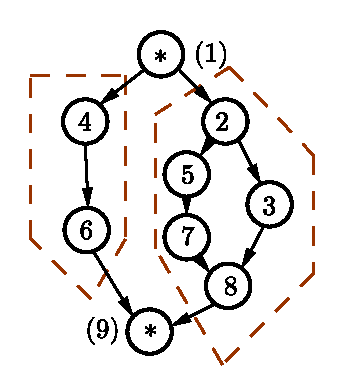
\includegraphics[width=.4\textwidth]{dag}
\end{subfigure}%
\caption{Ориентированный ациклический граф с возрастающими метками вдоль
путей.}
\label{fig:dag}	
\end{figure}

Вместе с оператором дифференцирования определён похожий по смыслу оператор
\textit{пометки}. Если задана экспоненциальная производящая функция
\[
    f(x) = \sum_{n \geq 0} a_n \dfrac{x^n}{n!} \enspace ,
\]
то
\[
    x \dfrac{d}{dx} f(x) = \sum_{n \geq 1} n a_n \dfrac{x^n}{n!} \enspace ,
\]
то есть коэффициент \( a_n \) заменяется на число \( n a_n \). Оператор пометки
можно определить на классах объектов, и его смысл заклчается в том, чтобы
выделить, пометить произвольно выбранный атом.
\begin{definition}
    Пусть \( F \)~--- класс объектов. Класс \( \point F \) состоит из объектов
вида \( (U, \theta) \), где \( \theta = (\gamma, u) \), \( \gamma \) является \(
F \)-структурой на \( U \), и атом \(u \in U \) интерпретируется как
\textit{выделенный элемент}.
\end{definition}

Например, если \( \mathfrak a \)~--- это класс \textit{деревьев}, то \(\mathcal A =
\point \mathfrak a \)~--- это класс \textit{корневых деревьев}.

\begin{example}[Формула Кэли]
    Деревья Кэли (подвешенные корневые деревья) \( A \) определяются соотношением на класс \( A \):
\[
    A = X \cdot \text{\textsc{set}}(A) \enspace .
\]
Рассмотрим класс \( \Pi \) \textit{позвоночных деревьев}, определённый как
\[
    \Pi = \point A \enspace .               
\]
Это означает, что кроме корня, теперь помечена ещё одна вершина 
(метки имеют разные цвета, скажем, красный цвет это корень, а синий цвет это
вторая пометка), и таким образом, дерево
оказалось <<подвешено>> на путь, соединяющий красную вершину с синей. Заметим,
что метки вершин в принципе могли совпасть, тогда одна вершина будет помечена
два раза. Из
определения класса деревьев следует, что в каждом дереве есть хотя бы одна
вершина, следовательно, класс позвоночных деревьев можно проинтерпретировать как
\[
    \Pi = \text{\textsc{seq}}_{\geq 1} (A) \enspace .
\]
Для производящих функций выполнено соотношение
\[
    \dfrac{1}{1-x} = \exp \left(
        \log \dfrac{1}{1 - x}
    \right), \quad
    \dfrac{x}{1-x} = \dfrac{1}{1 -x} - 1 =  \exp \left(
        \log \dfrac{1}{1 - x}
    \right) - 1 \enspace .
\]
Значит, помня о том, что производящая функция для класса \textsc{seq}$_{\geq 1}$
имеет вид \(\frac{x}{1-x}\), мы делаем вывод, что количество позвоночных
деревьев на \( n \) вершинах равно количеству \textit{множеств из циклов из
подвешенных деревьев} (см. рис. \ref{fig:composition})

Рассмотрим класс \textit{эндофункций}, который уже упоминался ранее по тексту:
это класс функций из \( \{ 1, 2, \ldots, n \} \to \{1, 2, \ldots, n\} \) для
всевозможных \( n \). Каждая эндофункция соответствует ориентированному графу, у
которого исходящая степень каждой вершины равна 1. Несложно показать, что любой
такой граф является множеством из циклов, где каждый элемент цикла является
корневым деревом.

Значит, количество позвоночных деревьев на \( n \) вершинах равно количеству
эндофункций на \( n \) атомах, то есть \( n^n \). Отсюда следует, что количество корневых деревьев
Кэли равно \( n^{n-1} \).
\end{example}

{\footnotesize
\textbf{Примечание}. Наверняка среди вас есть любители (например, я), которые
любят переделывать подобные доказательства в биективные, то есть которые не
требуют понятия производящей функции. Возникает естественное желание сравнить
полученное биективное доказательство с кодами Прюфера. По всей видимости,
алгоритм Прюфера делает нечто другое, а именно итеративно выбирает листовую вершину с
наибольшим номером, удаляет её, и записывает номер вершины, смежной с ней. Это
не эквивалентно приведенному выше доказательству, которое иллюстрирует другую
идею: если мы усложним задачу (пометим дополнительную вершину), то часто бывает
так, что решить её становится проще.

Кроме того, нужно подчеркнуть, что класс эндофункций не изоморфен классу
позвоночных деревьев, у них лишь совпадают экспоненциальные производящие
функции. Как мы помним, класс
\textsc{перестановок} не изоморфен классу \textsc{последовательностей}.}

Наконец, определим, как операторы дифференцирования и пометки действуют на
цикловом индексе, и как следствие, на обыкновенных производящих функциях.
\begin{theorem}
\[
    Z_{F'} = \dfrac{d}{dx_1} Z_F(x_1, x_2, x_3, \ldots), \quad
    Z_{\point F} = x_1 \dfrac{d}{d x_1} Z_F(x_1, x_2, x_3, \ldots). 
\]
Следовательно, для обыкновенной производящей функции выполнено
\[
    \widetilde{F'}(x) = \dfrac{d}{dx_1} Z_F(x, x^2, x^3, \ldots)\enspace ,
\quad
    \widetilde{\point F}(x) = x \dfrac{d}{dx_1} Z_F(x, x^2, x^3, \ldots)
\enspace .
\]
\end{theorem}
Доказательство теоремы~--- упражнение.
\subsection{Произведение Адамара}
Произведение Адамара на комбинаторном уровне, это покоэффициентное перемножение
для экспоненциальных производящих функций, и определено следующим образом:
\[
    \left(
        \sum_{n \geq 0} f_n \dfrac{x^n}{n!}
    \right) \bullet
    \left(
        \sum_{n \geq 0} g_n \dfrac{x^n}{n!}
    \right)  = 
    \sum_{n \geq 0} f_n g_n \dfrac{x^n}{n!} \enspace .
\]
Перед тем, как определить, как произведение Адамара действует на классах
объектов, небольшое отступление.
Обычно, под произведением Адамара понимают покоэффициентное произведение без
этих ваших факториалов:
\[
    \left(
        \sum_{n \geq 0} f_n x^n
    \right) \odot
    \left(
        \sum_{n \geq 0} g_n x^n
    \right)  =
    \sum_{n \geq 0} f_n g_n x^n \enspace , 
\]
В интернете у меня не получилось найти
ни одной сравнительной аналогии между этими двумя операторами, поэтому
приходится снова проводить самостоятельное журналистское расследование.
Начну с того, что свойства произведения \( \odot \) гораздо проще исследовать. Для произведения
<<точка-в-кружочке>> выполнен ряд теорем.
\begin{theorem}
    Если функции \( f(z) \) и \( g(z) \) аналитичны в нуле, то есть имеют
ненулевой радиус сходимости, то их произведение \( f(z) \odot g(z) \) тоже имеет
ненулевой радиус сходимости.
\end{theorem}
Заметьте, этого же нельзя сказать о произведении \( f(z) \bullet g(z) \)
(почему?), поэтому не всё так просто.
\begin{theorem}
Если \( f(z) \) и \( g(z) \) аналитичны в нуле, то для достаточно малых \( \rho
\) выполнено
    \[
    \sum_{n \geq 0} f_n g_n z^n = \dfrac{1}{2\pi i} \oint_{|\zeta| = \rho}
\dfrac{f(\zeta)}{\zeta} g \left( \dfrac{z}{\zeta} \right) d \zeta
    \enspace .
\]
\end{theorem}
\begin{proof}
Воспользуемся \textit{теоремой Коши о вычетах}. Обозначим \( [z^n]f(z) \)
коэффициент при \( z^n \) в разложении некоторой функции \( f(z) \). Тогда
\[
    [z^n] f(z) = \dfrac{1}{2\pi i} \oint_{|z| = \rho} \dfrac{f(z)}{z^{n+1}} dz
\enspace .
\]
Этот факт несложно доказать, раскладывая интеграл в сумму слагаемых, и кроме
того, его доказывают в самом начале курса по ТФКП. Используя теорему Коши,
получаем
\begin{multline*}
    \sum_{n \geq 0} f_n g_n z^n =
    \sum_{n \geq 0} \left(
        \dfrac{1}{2\pi i} \oint_{|\zeta| = \rho} \dfrac{f(\zeta)}{\zeta^{n+1}} d
    \zeta
    \right) b_n z^n
    = \\
    \dfrac{1}{2\pi i} \oint_{|\zeta| = \rho}
    \left(
        \dfrac{f(\zeta)}{\zeta} \sum_{n \geq 0} b_n \left( \dfrac{z}{\zeta}
    \right)^n
    \right) d \zeta = \dfrac{1}{2\pi i} \oint_{|\zeta| = \rho}
    \dfrac{f(\zeta)}{\zeta} g\left( \dfrac z \zeta \right) d \zeta \enspace .
\end{multline*}
\end{proof}
\begin{definition}
Рациональной функцией называется функция вида
\[
    f(z) = \dfrac{P(z)}{Q(z)} \enspace ,
\] 
где \( P(z) \) и \( Q(z) \)~--- многочлены. 
\end{definition}
\begin{theorem}
Если \( f(z) \), \( g(z) \)~---
рациональные функции, то \( f(z) \odot g(z) \) тоже рациональная функция.
\end{theorem}
\begin{proof}({\cite{lando}})
	Функция рациональна тогда и только тогда, когда существуют числа \( q_j \) и 
	многочлены \( p_j(n) \), что
	\[
		a_n = \sum p_j(n)q_j^n \enspace .
	\]
    Это легко доказывается разложением в сумму элементарных дробей. Значит,
коэффициент это сумму квазимногочленов.
	Произведение двух квазимногочленов является тоже квазимногочленом. Значит,
произведение Адамара двух рациональных функций рационально.
\end{proof}

Чтобы из оператора \( \odot \) получить оператор \( \bullet \), можно
рассмотреть \( f(z) \odot g(z) \odot \sum_{n \geq 0} n! z^n \). Такой вариант
весьма неудобен тем, что ряд \( \sum_{n \geq 0} n! z^n \) расходится, то есть не
аналитичен в нуле. В качестве альтернативного варианта можно воспользоваться
результатом задачи 1 из семинара 1, превратив экспоненциальную производящую
функцию в обыкновенную (без гарантии, что аналитичность сохранится), и взять
произведение Адамара для результирующей функции. Таким образом, получаем формулу
\[
    f(z) \bullet g(z) = \widetilde f(z) \odot g(z), \quad
    \widetilde f(z) = \int_{0}^\infty e^{-y} f(yz) dy \enspace ,
\]
\[
    f(z) \bullet g(z) = \dfrac{1}{2\pi i} \oint_{|\zeta| = \rho}
    \int_{0}^\infty e^{-y} f(y \zeta) \cdot g \left(\dfrac{z}{\zeta} \right)
\dfrac{dy\; d \zeta}{\zeta}
\enspace .
\]
Ещё раз подчеркну, что во-первых, формула не всегда верна (только, когда
соответствующие функции аналитичны), а во-вторых, тильдочка над \( f(z) \) не
означает переход к непомеченным объектам. Простым стиранием факториалов этого
нельзя добиться.

Формулы, которые мы сейчас получили, могут пригодиться для изучения асимптотики
коэффициентов некоторых производящих функций. Один из примеров разобран в
\cite[Example VI.14, page 425]{AC}: пьяница передвигается по \( \mathbb Z^d \),
передвигаясь по каждой координате на \( \pm 1 \) независимо с вероятностью \(
1/2 \). Для получения асимптотики коэффициентов используются свойства
сингулярностей произведения Адамара производящих функций.

Перейдём к определению комбинаторного произведения Адамара для классов объектов.
\begin{definition}
    Пусть \( F \), \( G\)~--- два класса объектов. Класс \( F \bullet G \)
называется \textit{произведением Адамара} классов \( F \) и \( G \), и состоит
из объектов вида \( (U, \theta) \), где \( \theta = (\alpha, \beta) \), причём
\(\alpha \) является \(F\)-структурой над \(U \), \(\beta\) является
\(G\)-структурой над \( U \).
\end{definition}
Ответим на вопрос: в чём заключается различие произведения Адамара от обычного
декартова произведения? Если мы рассмотрим, скажем, декартово произведение
деревьев и циклов, то объект размера \( 7 \) может состоять например из 4
атомов, объединённых в дерево, и 3 атомо, объединённых в цикл, тогда как для
произведения Адамара имеется 7 атомов, на которых задана одновременно и
структура дерева и структура цикла.

{\footnotesize
\textbf{Примечание.} Рекомендую заглянуть в немного юмористическую, на мой
взгляд, заметку о теории категорий и производящих функцях
(мне понравилась аналогия про декатегорификацию стада овец): From Finite Sets to Feynman Diagrams
\cite{category_feynman}. Лозунг статьи в том, чтобы рассматривать изоморфизмы
вместо равенств. Оказывается, что произведение Адамара (inner product)
там играет роль категорификатора для Гильбертова пространства квантового
гармонического осциллятора. (испугались?)
}

\begin{example}[Циклы, снабжённые подмножествами]
Рассмотрим класс \( \mathcal C \) циклов и \( \mathfrak p \) подмножеств. Их
произведение Адамара имеет экспоненциальную производящую функцию  \( \log \left(
\dfrac{1}{1 - 2x} \right) \). Действительно, количество циклов на \( n \)
элементах равно \( (n-1)! \), а количество подмножеств \( 2^n \). Значит, ЭПФ
имеет вид
\[
    \sum_{n \geq 1} (n-1)! 2^n\dfrac{x^n}{n!} = \log 1/(1-2x) \enspace .
\]
\end{example}

Напомню, что через \( \mathbf{aut}(\sigma) \) мы обозначили количество
перестановок, сопряжённых с данной, и это число можно найти, зная цикловой тип
перестановки \( \sigma \):
\[
    \mathbf{aut}(\sigma) = 1^{\sigma_1} \sigma_1! 2^{\sigma_2} \sigma_2!
3^{\sigma_3} \sigma_3 ! \ldots \enspace .
\]

\begin{theorem}
    Пусть заданы классы \( F \) и \( G \). Их цикловые индексы имеют вид
\[
    Z_F(x_1, x_2, x_3, \ldots) = \sum_{\vec n} f_{\vec n} \dfrac{\vec x^{\vec
n}}{\mathbf{aut}(\vec n)} \enspace , \quad
    Z_G(x_1, x_2, x_3, \ldots) = \sum_{\vec n} g_{\vec n} \dfrac{\vec x^{\vec
n}}{\mathbf{aut}(\vec n)} \enspace .
\]
Тогда цикловой индекс для их произведения
Адамара имеет вид
\[
    Z_{F \bullet G} = \sum_{\vec n} f_n g_n \dfrac{\vec x^{\vec
n}}{\mathbf{aut}(\vec n)} \enspace . 
\] 
\end{theorem}

\subsection{Функториальная композиция}
Вот мы и подошли к финальной операции, а именно функториальной композиции. Такое
название она получила из-за того, что теория классов объектов возникла
естественным образом как применение теории категорий к аппарату производящих
функций. С точки зрения теории категорий, \textit{класс объектов} является
функтором от множества атомов, поэтому если представить функтор как множество
атомов, и построить на нём другой функтор, то получится \textit{функториальная
композиция}.

\begin{definition}
    Пусть \( F \) и \( G \)~--- два класса объектов. Класс \( F \fprod G \) 
называется \textit{функториальной композицией} классов \( F \) и \( G \) и
состоит из объектов \( (U, \theta) \), где \( \theta \) является структурой типа
\( F \) над множеством \( G[U] \) всевозможных структур над \( U \).
\end{definition}

\begin{example}
    Пусть \( \mathfrak p \)~--- класс \textit{подмножеств}, \( \mathfrak p^{[2]}
\)~--- класс подмножеств размера 2.
    С помощью функториальной композиции можно построить класс \textit{простых
графов} \( \mathcal G \), заданный формулой
\[
    \mathfrak p \fprod \mathfrak p^{[2]}
    \enspace  .
\]
Если задано множество атомов \( U = \{1, 2, \ldots, n \} \), то оно играет роль
множества вершин. Двухэлементное подмножество множества вершин это ребро графа.
Если рассматривать все \( {n \choose 2} \) возможных рёбер как <<новые атомы>>,
то подмножество рёбер задаёт те рёбра, которые нарисованы в данном графе.
\end{example}

В чём различие между функториальной композицией и обычной композицией? Мы с вами
сейчас точно знаем, что функториальная композиция~--- это операция из эдакого
магического мира, потому что она позволяет из двух классов с не очень быстрым
ростом коэффициентов получить класс, в котором коэффициенты растут настолько
быстро, что производящие функции имеют нулевой радиус сходимости.

Если мы рассматриваем обычную композицию \( F \circ G \), и объект на \( n \)
атомах, то \( n \) представляется в виде суммы нескольких слагаемых, и \( G
\)-структура строится отдельно на каждом из слагаемых. Напротив, в
функториальной композиции каждый атом задействован сразу в нескольких структурах
(вершина графа может быть инцидентна сразу нескольким рёбрам), отсюда и увеличение
числа возможных структур.

Предположим, что для каждого \( n \in \mathbb N \) существует хотя бы одна \( G
\)-структура над \( \{1,2,\ldots, n\} \). Тогда ЭПФ функториальной композиции
имеет вид
\[
    \left(
    \sum_{n \geq 0} f_n \dfrac{x^n}{n!}
    \right)
    \fprod
    \left(
    \sum_{n \geq 0} g_n \dfrac{x^n}{n!}
    \right)
    = 
    \sum_{n \geq 0} f_{g_n} \dfrac{x^n}{n!} \enspace .
\]
Эта формула выглядит довольно невероятной. Кроме того, можно получить выражение
для циклового индекса функториальной композиции. Для этого нужно снова немного
порефлексировать над определением циклового индекса. Вспомним пример с
инволюциями. В определении фигурирует \(
\mathrm{Fix}\;F[\sigma]\), что означает количество неподвижных точек в
перестановке объектов \( F[U] \), индуцированной перестановкой \( \sigma \). Для
того, чтобы знать, как 26 инволюций переходят друг в друга, не обязательно знать
перестановку~--- достаточно знать лишь её цикловой тип.

Если имеется перестановка \(\sigma \) и класс \( G \), то \( (G[\sigma])_1 \)
это количество неподвижных точек перестановки \( G[\sigma] \), \( (G[\sigma])_2
\)~--- количество 2-циклов, и так далее.

\begin{theorem}
    Функториальная композиция для цикловых индексов определяется формулой
\[
    Z_F \fprod Z_G = \sum_{n \geq 0 } \dfrac{1}{n!} \sum_{\sigma \in S_n}
    \mathrm{Fix}\; F[(G[\sigma])_1, (G[\sigma])_2,
\ldots]x_1^{\sigma_1}x_2^{\sigma_2} \ldots
\]
\end{theorem}

\section{Задачи}

\begin{enumerate}
	\item(1 очко) На семинаре Эдуард предложил рекуррентное 
	соотношение для числа инволюций вида
	\[
		I_{n} = I_{n-1} + (n-1)I_{n-2} \enspace ,
	\]
	мотивируя это тем, 
	что 
	максимальный элемент можно либо зациклить с самим собой (оставшиеся \( n-1 
	\) 
	элементов образуют инволюцию), либо с каким-то из других \( (n-1) \) 
	элементов, 
	при этом остаётся \( (n-2) \) элемента, которые опять таки образуют 
	инволюцию.
	
	Проверьте, выполнено ли это соотношение, и если да, напишите 
	соответствующее 
	соотношение для экспоненциальных производящих функций, а затем глядя на 
	него, 
	придумайте (рекуррентное) соотношение для класса инволюций \( \mathrm{Inv} 
	\).
    \item(2 очка) Найдите сумму 
    \[
        \sum_{k = 0}^{\infty} {n \choose 3k}
    \]

	\item(0 + 1 + 1 очко) Докажите формулы для цикловых индексов \( Z_L, Z_P,
Z_S \). Воспользуйтесь обозначением \( \mathbf{aut}(\sigma) \) и альтернативным
выражением для циклового индекса.
	\item(1 + 1 + 1 очко) \textbf{Алгебраические свойства.}
        \begin{enumerate}
        \item	Докажите, что класс pointed sets \( \point E \) является 
        нейтральным элементов для операции функториальной композиции
        \[
            F \fprod \point E = \point E \fprod F = F \enspace .
        \]
        \item Произведение Адамара можно выразить с помощью декартова произведения 
        и оператора \( \fprod \).
        \item 
\[
	(F \bullet G) \fprod H = (F \fprod H) \bullet (G \fprod H)
\]
        \end{enumerate}
	\item(1 очко) Докажите, что класс ориентированных графов можно задать как 
	\[
		D = \mathfrak p \fprod (\point E \bullet \point E)
	\]
    \item(4 очка) Пусть \( \varphi(k) \)~--- функция Эйлера.
\[
    \dfrac{x}{1-x} = \sum_{k \geq 1} \dfrac{\varphi(k)}{k} \log \dfrac{1}{1 -
x^k} \enspace.
\]
	\item(3 очка) Покажите, что для класса \( \mathcal V \) позвоночных деревьев
и \( \mathcal A \) корневых деревьев выполнено соотношение
\[
    \mathcal V = \mathcal A + \mathcal V \times \mathcal A \enspace .
\]
Докажите для \( n \geq 1 \) тождество 
\[
    n^n = \sum_{k = 0}^{n-1} {n \choose k} k^k (n-k)^{n-k-1} \enspace .
\]
    \item(1 очко) Найдите произведение Адамара \( (1 - rx)^{-1} \odot (1 - sx)^{-1}\).
    \item(2 очкa) Пусть \( \mathfrak p \)~--- класс подмножеств, \( \beta\)~---
некоторая перестановка. Докажите, что
    \[
    \mathrm{Fix}\; \mathfrak p [\beta] = 2^{\sum_{k \geq 1} \beta_k} \enspace ,
    \]
где $(\beta_1, \beta_2, \ldots)$~--- цикловой тип перестановки \( \beta \).
\end{enumerate}

\footnotesize
\bibliographystyle{plain}
\bibliography{biblio}
    
\end{document}
